\documentclass{article}
\usepackage[pdftex]{color}
\usepackage{graphicx}
\begin{document}

\def\path#1{#1}

\long\def\issue#1{{\color{red} #1}}

\section{Building Cardioid}

This section migrated to doxygen

\section{Command Line Arguments}

This section migrated to doxygen (running cardioid page)

\section{Input Files}

The input parameters for a Cardioid job are read from the files
\path{object.data} and, if it is present, \path{restart}.  These two
files consists of a number of ``object'' blocks that can be used to
control all aspects of the job.

An object block is of the form
\begin{verbatim}
name ClassName { 
  keyword1 = value1; 
  keyword2 = value2;
  keyword3 = value3.1 value3.2 value3.3;
  ...
}
\end{verbatim}
Values may be string, floats, or integers and may be vector or scalar
valued.  Units are supported.  The set of keywords is open and
arbitrary.  Both C and C++ style comments are supported.  All
identifiers are case sensitive.  The order of objects in the file is
arbitrary.  If two objects with the same name and class name appear in
the file they are treated as if the keyword value lists are
concatenated.  If the same keyword appears multiple times within a
single object the last value overrides all others.  By convention,
object names are mixed case, class names are all caps.


The primary or root object in the \path{object.data} file is the
SIMULATE object and the job is configured according to its settings.  A
complete list of the supported object classes and their keywords is
given in the appendix.

The \path{restart} file is typically present only when restarting jobs
from a checkpoint file.  The \path{restart} file is generated
automatically along with a checkpoint file and is always read after the
\path{object.data} file.  This order is important because it allows the
\path{restart} file to override certain settings that change over the
course of the simulation such as the time and loop count.  It also
contains the location of the checkpoint file.  One way to think of the
relationship between \path{object.data} and \path{restart} is that
\path{object.data} contains parameters that do not change as the
simulation progreses while \path{restart} contains those that do.

\subsection{Conventions for Input Files}

When Cardioid writes files with large amounts of data (such as
checkpoint or visualization files) it uses the pio system described in
section~\ref{sec:pio}.  Pio files are always written in snapshot
directories.  A snapshot directory is named \path{snapshot.xxxxxxxx}
where \path{xxxxxxxx} is the value of the simulation loop counter when
the directory was created.  The \path{restart} file that corresponds to
a checkpoint file written in the corresponding snapshot directory and a
symbolic link to the restart file are created in the run directory.  Each
time a new checkpoint file is written the link is updated to point at
the most recent restart file.  You can easily change which checkpoint
file you want to use for restart by pointing the symbolic link at the 
\path{restart} file in the corresponding snapshot directory.

Here are some suggested best practices that will help organize files.
\begin{enumerate}
\item  Place all pio style files (anatomy, state, etc) in a snapshot
  directory.  This applies even to files that are created by tools other
  than Cardioid.  Frequently we use the directory
  \path{snapshot.initial} to hold the files that are used to initialize
  the simulation.  Do not use \path{snapshot.00000000} for this purpose
  as Cardioid may overwrite files in any numbered snapshot directory.
\item Never place an actual file named \path{restart} in the run
  directory.  Use only symbolic links (created with the command ln -s)
  that point to actual files someplace else (such as in a snapshot
  directory).  Cardioid deletes the old \path{restart} file in the run
  directory each time it creates a new checkpoint file.  Using symbolic
  links assures that no actual data will be deleted, only pointers to
  the data.
\end{enumerate}


\section{Units}

Values in the input deck may include a unit specification.  For reasons
of clarity, units are strongly encouraged.  

Because standard unit systems such as MKS and cgs are not convenient for
electrophysiolgy simulation, Cardioid defines a custom unit system.
In this system the seven fundamental units are:
\begin{description}
\item[length] millimeter
\item[mass]   microgram
\item[time] millisecond
\item[current] milliamp
\item[temperature] Kelvin
\item[amount] nanomol
\item[luminous intensity] candella
\end{description}
Derived units follow from these seven fundamentals.  For example, the
dimensionality of voltage is 
\[
voltage = \frac{mass * length^2}{current * time^3} 
\]
Substituting our base units we obtain
\[
\frac{ug*mm^2}{mA*ms^3} = \frac{10^{-15}}{10^{-12}}\frac{kg*m^2}{A*sec^3} =
10^{-3}volts
\]
Hence the unit for voltage is millivolts.  The default units for typical
quantities of interest include
\begin{description}
\item[voltage] millivolt
\item[capacitance] millifarad
\item[conductivity] siemen
\item[charge] microcoulomb
\item[concentration] millimolar
\end{description}
Internally all quanties are represented in this unit system.  When no
unit is specified, all quantities in the input deck are assumed to be in
these units.

The usual unit rules do not apply to code in the cell models.  Code in
the cell models may come from other sources (such as CellML) that use
different unit conventions.  Use caution.

\subsubsection{Supported Units}

Supported units are as follows:
\begin{description}
\item[Length] meter, mm, um, nm.  (Do not use ``m'' for meter.)
\item[Mass] gram, g, kg, mg, ug.
\item[Time] second, s, ms, us, ns, ps, fs.  (Do not use sec.)
\item[Current] amp, A, mA, uA.
\item[Temperature] K.
\item[Voltage] volt, V, mV, uV.
\item[Capacitance] farad, F, mF, uF, nF, pF.
\item[Resistivity] siemens, S, mS, uS.
\item[Charge] coulomb, C, mC, uC.
\end{description}


\subsubsection{Examples}

Here are several examples of valid unit specifications:

\begin{verbatim}
diffusionScale = 714 mm^3/mF;
dx = 0.1 mm;
sigmaLi = 0.3 mS/mm;
sigmaLi = 0.0003 S/mm;
dt =0.01 ms;
vSitm = -52 mV/ms;
\end{verbatim}

\subsubsection{Limitations}

\begin{enumerate}
\item For tecnical reasons, ``m'' is not a valid specification for
  ``meter''.  You may use meter, mm, um, and nm.
  \item The unit parser is limited in the expressions it can handle.
    Expressions may contain multiplication (*), division (/) and
    exponentiation (\^) with integer valued exponents both positive and
    negative.  It cannot handle parentheses.  
\end{enumerate}

Given the limitations above, here are a few more examples showing right
and wrong ways to specify complex units.
\begin{verbatim}
voltage = 1 V;
voltage = 1 volt;
voltage = 1 kg*m^2/A/s^3;       // Invalid.  Don't use m for meter.
voltage = 1 kg*meter^2/(A*s^3); // Invalid.  Parentheses not allowed.
voltage = 1 kg*meter^2/A/s^3;
voltage = 1 kg*meter^2*A^-1*s^-3;
\end{verbatim}


\appendix

\section{Object Classes}

\newenvironment{keywords}
{
  \par\vspace{12pt}\noindent
  \begin{tabular}{|r|p{0.7\textwidth}|}
    \hline
    Keyword & Description \\ \hline
  }
  {
  \end{tabular}\par
}

\def\kw#1#2#3{%
  #1 & {#2 \par Default: #3}\\ \hline%
}


\subsection{ANATOMY}

\subsubsection{Coordinate system}

Moved to Doxygen

\subsubsection{brick method}

Moved to Doxygen

\subsubsection{pio method}

Moved to Doxygen
 

\subsubsection{Conductivity}
Note: prior to r261 the name of the CONDUCTIVITY object was specified in
the DIFFUSION object.  Input of Conductivity tensors and floating point
fibre angles are not supported prior to r261.

There are several ways to specify the conductivity tensors for each cell
in the anatomy.  The most direct method is to include the conductivity
tensor in the anatomy file.  Note that the units of the tensor elements
must be specified in the header and must have the dimensionality of
resistivity/length.  (Section~\ref{sec:AnatomyFormat} contains a description
of the anatomy file contents.)  When the tensor is present in the
anatomy file no other conductity specification is necessary.  If any
other specification is present it may override the tensor values in the
anatomy file.

If no tensor data is present in the file, a CONDUCTIVITY object that
specifies a method such as ``uniform'' or ``fibre'' must be present in
the ANATOMY object.



\begin{verbatim}
pioAnatomy ANATOMY 
{
   method = pio;
   fileName = snapshot.initial/anatomy#;
   dx = 0.167;   // in mm
   dy = 0.167;   // in mm
   dz = 0.167;   // in mm
}
\end{verbatim}

\subsection{CONDUCTIVITY}
\begin{keywords}
  \kw{method}{Choose from ``pio'', ``fibre'', ``JHU'' or
    ``uniform''}{``pio''}
\end{keywords}

\subsubsection{pio}
The conductivity tensor will be read from the input anatomy file.

\subsubsection{fibre}
The conductivity tensor will be generated from the fibre angles
given in the anatomy and the longitudinal and transverse
conductivities.  If the anatomy does not provide fibre angles, then the
values 0, 0 are assumed for all cells.
\begin{keywords}
  \kw{sigmaLi}{Longitudinal conductivity (i.e., in the direction of the
    fibre) in Siemens/mm.}{0.3e-3~S/mm} 
  \kw{sigmaTi}{Transverse conductivity (i.e., perpendicular to the
    direction of the fibre) in Siemens/mm}{0.0315e-3~S/mm}
\end{keywords}
\issue{Check that the units really are Siemens/mm.  If so, these aren't
  very good default values.}
\subsubsection{JHU}
\begin{keywords}
  \kw{homogeneousFiber}{}{0}
  \kw{rotationMatrix}{}{1}
  \kw{sigmaLi}{}{0.3e-3}
  \kw{sigmaTi}{}{0.0315e-3}
  \kw{sheetAngle}{}{45}
\end{keywords}

\subsubsection{uniform} 
A specified tensor for all cells.  All components are given in Siemens/mm.
\begin{keywords}
  \kw{sigma11}{Component of the conductivity tensor.}{0.1e-3~S/mm}
  \kw{sigma22}{Component of the conductivity tensor.}{0.1e-3~S/mm}
  \kw{sigma33}{Component of the conductivity tensor.}{0.1e-3~S/mm}
  \kw{sigma12}{Component of the conductivity tensor.}{0.0~S/mm}
  \kw{sigma13}{Component of the conductivity tensor.}{0.0~S/mm}
  \kw{sigma23}{Component of the conductivity tensor.}{0.0~S/mm}
\end{keywords}


\subsection{DECOMPOSITION}
\begin{keywords}
  \kw{printStats}{}{0}
\end{keywords}

\subsection{DIFFUSION}

\begin{keywords}
  \kw{method}{Choose from ``FGR'', or ``null''.  Saleheen methods are no
  longer supported.}
  {Default: FGR}
  \kw{diffusionScale}{An overall scaling factor applied to $dV/dt$
    computed by the diffusion solver.  Presently, it is used to account
    for the membrane capacitance and surface to volume ratio.  The value
    should be set to $1/(S*C_m)$ where $S$ is the surface to volume ratio
    in mm$^{-1}$ and $C_m$ is the membrane capacitance per unit area in
    mF/mm$^2$. 
    \issue{The default is not a very sensible value}}{1 mm$^3$/mF}
\end{keywords}


Example:
Assuming $C_m = 0.01~\mu$F/mm$^2$ and $S=140$~mm$^{-1}$
\begin{verbatim}
fgr DIFFUSION
{
   method = FGR;
   diffusionScale = 714.285; // mm^3/mF
}
\end{verbatim}

Note: Starting from r261 the conductivity is no longer specified in the
DIFFUSION object but rather in the ANATOMY object.

\subsection{REACTION}
A variety of tissue models are available to calcuate the reaction terms:

\begin{description}
  \item[TT04\_CellML] TT04 model straight from the code generated by
    CellML.  Code is written for absolute fidelity to the generated
    code, not for performance.
  \item[TT06\_CellML] TT06 model straight from the code generated by
    CellML.  Code is written for absolute fidelity to the generated
    code, not for performance.
  \item[TT06Dev] Developmental version of TT06 with Pade approximations,
    optimizations, etc.
  \item[TT06\_RRG] TT06 based on CellML with added Na equation from
    Jeremy.  Some parameters can be set on a cell-by-bell basis.
  \item[FHN] FitzHugh Nagumo model.
  \item[test] 
  \item[null] No reaction model is computed
\end{description}



\begin{keywords}
  \kw{method}{Choose from: TT04\_CellML, TT06\_CellML, TT06Dev,
    TT06\_RRG, FHN, null}{No default}
\end{keywords}


\subsection{SENSOR}

Used to write values of interest to a file.

\issue{At present the sensors are limited to quantities related to
  membrane voltage.  A significant limitation is they cannot print any
  of the internal state variables of the reaction model.  This will be
  fixed in a future version.}

\begin{keywords}
  \kw{evalRate}{Rate in time steps at which the sensor eval function is called.}{1}
  \kw{method}{Choose from ``pointList'', ``activationTime'', ``maxDV''
    ``dataVoronoiCoarsening'' and ``gradientVoronoiCoarsening''.}{No
    default}
  \kw{printRate}{Rate in time steps at which the sensor print
    function is called.}{1}
\end{keywords}

\subsubsection{PointList Sensor}
Prints information at points specified by grid index.  The evalRate is
ignored for this sensor.
\begin{keywords}
  \kw{dirname}{Directory in which output files are written.}{sensorData}
  \kw{endTime}{For time $>$ endTime sensor prints nothing.  Negative value
    implies no endTime.}{-1~msec}
  \kw{filename}{Base name for output file.  Each cell is written to a
    separate file with its grid index appended to this name.}{cell}
  \kw{pointList}{List of grid coordinates of cells to print values}{No
    Default}
  \kw{printDerivs}{Set to non-zero value to activate printing of certain
    derivatives of the membrane voltage}{0}
  \kw{startTime}{For time$<$startTime sensor prints nothing}{0~msec}
  
\end{keywords}

\subsubsection{dataVoronoiCoarsening Sensor}
Prints $V_m$ at points specified by grid indexes. 
The values are obtained by averaging over the Voronoi cell associated to each point.

The evalRate is ignored for this sensor.

\begin{keywords}
  \kw{cellList}{Name of file containing list of grid coordinates of cells to print values}{No
    Default}
  \kw{filename}{Base name for output file.}{``coarsened\_anatomy''}
\end{keywords}

\subsubsection{gradientVoronoiCoarsening Sensor}
Prints $\nabla V_m$ at points specified by grid indexes. 
The values of $\nabla V_m$ at a point $x_0$ is
obtained by solving a linear least squares system
$$
X^TW^2 X \nabla V_m=W {\bf b}
$$
where $X$ is a $k\times 3$ matrix whose rows are the positions vectors 
for each of the $k$ points in the Voronoi cell with respect to the point where
$\nabla V_M$ is to be evaluated, that is $(x_k-x_0)^T$,
${\bf b}$ is the k-dimensional vector made of the differences $V_m(x_k)-V_m(x_0)$,
and $W$ is a $k\times k$ diagonal matrix with diagonal elements given by $w_i=1/\|x_i-x_0\|$.

The evalRate is ignored for this sensor.

\begin{keywords}
  \kw{cellList}{Name of file containing list of grid coordinates of cells to print values}{No
    Default}
  \kw{filename}{Base name for output file.}{``coarsened\_anatomy''}
\end{keywords}

\subsubsection{maxDV Sensor}
Prints the minimum and maximum value of $dV_m/dt$ over all active cells.
The evalRate is ignored for this sensor.

\begin{keywords}
  \kw{filename}{Name for output file.}{``stdout''}
\end{keywords}

\subsection{SIMULATE}

Moved To Doxygen

\subsection{STIMULUS}

Specifies an external stimulus current that is applied to a cell or
group of cells.  

\begin{keywords}
  \kw{method}{Choose from ``box'', ``point'', or ``test''}{No default.}
  \kw{pulse}{Choose from ``periodic'', or ``random''}{``periodic''}
  \kw{t0}{Specifies a time before which the simulus is zero.  Regardless
    of all other parameter values, at all
    $t<t0$ the stimulus current is zero.}{-1000~msec}
  \kw{tf}{Specifies a time after which the simulus is zero.  Regardless
    of all other parameter values, at all
    $t>tf$ the stimulus current is zero.}{$10^{30}$~msec}
\end{keywords}

\subsubsection{Periodic Pulse Trains}
\label{sssec:pulseTrains}
Many of the stimulus methods apply a periodic square wave pulse train
(See Figure~\ref{fig:pulseTrain}) to selected cells.  They share a
common set of keywords to specify the pulse train.  These keywords are:
\begin{keywords}
  \kw{duration}{The length of time the stimulus is on (in msec).}{1~msec}  
  \kw{period}{The period of the pulse train (in msec).}{1000~msec}  
  \kw{tStart}{The delay from the start of each period to start the
    simulus (in msec).  This parameter sets the phase of the wave.}{0.}
  \kw{vStim}{The amplitude of the stimulus (in mV/msec).  This value is
    negative by convention to specify depolarization.  A negative vStim
    corresponds to a positive $dV/dt$.}{Varies with method.}
\end{keywords}

\begin{figure}
  {\centering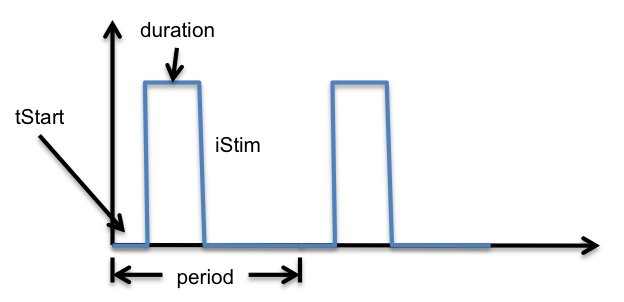
\includegraphics{graphics/pulseTrain.png}}
  \caption{Periodic pulse train.}
  \label{fig:pulseTrain}
\end{figure}

\subsubsection{Random Period Pulses}
\label{sssec:randomPeriodPulse}
This option shares most of the options with the periodic pulse train.
The only difference is that it uses a 'min' and 'max' period instead of a single and constant period.
The keywords are:
\begin{keywords}
  \kw{min\_period}{The minimum length period of the pulse train (in msec).}{1000~msec} 
  \kw{max\_period}{The maximum length period of the pulse train (in msec).}{1000~msec} 
\end{keywords}
Every time a period ends, a new period length will be randomly picked 
in a uniform probability distribution between 'min\_period' and 'max\_period'.

\issue{Jeremy has indicated that it is more natural to specify the
  stimulus current in units of current/volume rather than the stimulus
  voltage.  We will add an iStim keyword in a future version.}

\issue{The behavior of multiple STIMULUS objects is not carefully
  implemented.  Should it always be the sum?}

\issue{As implemented, the Stimulus class can access and modify the
  value of $dV/dt$ due to diffusion.  This is a carry over from
  BlueBeats.  Is this a good idea?  Should we eliminate this possiblity?
   Should it be under keyword control?  Note that this imposes some
   potentially undesirable serialization constraints.}

\subsubsection{Box Stimulus}

Applies the stimulus to all cells inside a specified box.  \issue{The
  concept of inside a specified box is vague, especially since the cell
  can only be stimulated at a discretization point.  What about points
  that are on the boundary?  Should there be some kind of integration of
  the amount of volume associated with the point that is inside the box?
  This is closely related to the issue that the layout of the
  discretization in the box method for ANATOMY is not well defined.}

\begin{keywords}
  \kw{duration}{See Section~\ref{sssec:pulseTrains}.}{1~msec}
  \kw{period}{See Section~\ref{sssec:pulseTrains}.}{1000~msec}
  \kw{tStart}{See Section~\ref{sssec:pulseTrains}.}{0~msec}
  \kw{vStim}{See Section~\ref{sssec:pulseTrains}.}{-52~mV/msec}
  \kw{xMin}{Minimum grid index in the $x$-direction to stimulate.}{-1}
  \kw{xMax}{Maximum grid index in the $x$-direction to stimulate.}{Size of global grid in $x$-direction.}
  \kw{yMin}{Minimum grid index in the $y$-direction to stimulate.}{-1}
  \kw{yMax}{Maximum grid index in the $y$-direction to stimulate.}{Size of global grid in $y$-direction.}
  \kw{zMin}{Minimum grid index in the $z$-direction to stimulate.}{-1}
  \kw{zMax}{Maximum grid index in the $z$-direction to stimulate.}{Size of global grid in $z$-direction.}
\end{keywords}

\issue{Isn't it awkward that we specify the box in units of grid cells?
  Should it be in length units (like mm) instead?}

  Only cells
that are strictly inside the box are stimulated.  Cells with indices
that are equal to the min or max index are not stimulated.  For example,
setting xMin=1, xMax=3 will stimulate cells with ix=2.

\subsubsection{Point Stimulus}
Applies the stimulus to a single cell specified by its global grid index.

\begin{keywords}
  \kw{cell}{The global grid index of the cell to stimulate.  See
    Section~\ref{sec:AnatomyFormat} for an explanation of the global grid
  index.}{0}
  \kw{duration}{See Section~\ref{sssec:pulseTrains}.}{1~msec}
  \kw{period}{See Section~\ref{sssec:pulseTrains}.}{1000~msec}
  \kw{tStart}{See Section~\ref{sssec:pulseTrains}.}{0~msec}
  \kw{vStim}{See Section~\ref{sssec:pulseTrains}.}{-52~mV/msec}
\end{keywords}

\subsubsection{Test Stimulus}
Intended for testing only.  Applies stimulus to a single cell specified
by a local index and an MPI rank.

\begin{keywords}
  \kw{cell}{The local index of the cell to stimulate.}{0}
  \kw{duration}{See Section~\ref{sssec:pulseTrains}.}{1~msec}
  \kw{period}{See Section~\ref{sssec:pulseTrains}.}{1000~msec}
  \kw{rank}{The MPI rank of the cell to stimulate.}{0}
  \kw{tStart}{See Section~\ref{sssec:pulseTrains}.}{1~msec}
  \kw{vStim}{See Section~\ref{sssec:pulseTrains}.}{-52~mV/msec}
\end{keywords}


\section{Pio Files}
\label{sec:pio}

Cardioid reads and writes large files such as anatomy, visualization, or
state files using a parallel I/O system known as ``pio.''  The pio
system is designed to provide extremely high I/O performance on a
variety of machines.  Because file-per-task and file-per-job approaches
to parallel I/O both have serious problems at large scale we take a
middle road and divide the data into $n$ physical files where $n$ is
typically in the range of 1--2000.  For very large scale jobs and
highest throughput $n$ can be tuned according to the number of I/O nodes
on the system or some other hardware parameter that limits performance
such as the number of storage targets.


The filenames of the $n$ physical files in a pio logical file all share
common base name and end with the \#-sign and a six digit sequence
number.  For example, anatomy\#000000, anatomy\#000001, \ldots You can
think of this set of files as being logically concatenated in numerical
order.  Pio files may contain either ascii or binary data.

The zeroth file contains a human readable ascii header that describes
the data.  This header is of the form
\begin{verbatim}
name ClassName { 
  keyword1 = value1; 
  keyword2 = value2;
  ...
}
\end{verbatim}
Note that this is exactly the same form as an object in the object.data
input file.  Values may be string, floats, or integers and may be vector
or scalar valued.  Units are supported.  The set of keywords is open and
arbitrary.  You can put whatever data you want in the header to help
identify the file.  The maximum header length is something like 4k but
that could be easily extended if it became a limitation.  The header
ends with two newline characters in a row.  

An example header for an ascii pio file looks like this:
\begin{verbatim}
anatomy FILEHEADER{
  datatype = FIXRECORDASCII;
  nfiles = 1;
  nfields = 4;
  field_names = gid cellType theta phi;
  field_types = u u f f;
  nx = 3; ny = 3; nz = 3;
  nrecord = 27;
  lrec=12;
}
\end{verbatim}

Most of the  keywords in the header represent metadata that describe the
structure of the files and the data they contain.  This metadata is used
by both the pio system to read the files correctly and by various other
routines to understand how to load data into memory.

\issue{There should be a keyword table here that lists the pio keywords.}



\section{Anatomy File Format}
\label{sec:AnatomyFormat}

All I/O of anatomy files is handled by the pio system described in
Section~\ref{sec:pio}.  
An example header for an ascii anatomy file looks like this:
\issue{This could be a more realistic example such as for a file with
  conductivities.  It would contain units etc.}
\begin{verbatim}
  anatomy FILEHEADER{
  datatype = FIXRECORDASCII;
  nfiles = 1;
  nfields = 4;
  field_names = gid cellType theta phi;
  field_types = u u f f;
  nx = 3; ny = 3; nz = 3;
  nrecord = 27;
  lrec=12;
}
\end{verbatim}

The meaning of most of the keywords should be fairly self-evident.
\issue{However, this documentation should describe them and specify
  which keywords are manditory.}  Most are needed by pio to determine
how to read the file.  \issue{For now we're using ascii to facilitate
  debugging.  Binary files will be available in the future to improve
  performance and decrease storage cost.}


\bigskip
The allowed field names and corrsponding field types are as follows:

\begin{tabular}{l|l|l|p{.6\textwidth}}
  & & & \\
  Field Name & Field Type & Required? & Description\\
  \hline
  gid &      8-byte integer   & Required & Cell index (described below)\\
  cellType & integer          & Required & Cell type (described below)\\
  theta &    integer or float & Optional & Polar angle of fibre\\
  phi &      integer or float & Optional & Azimuthal angle of fibre\\
  sigma11 &  float            & Optional & Component of conductivity tensor\\
  sigma22 &  float            & Optional & Component of conductivity tensor\\
  sigma33 &  float            & Optional & Component of conductivity tensor\\
  sigma12 &  float            & Optional & Component of conductivity tensor\\
  sigma13 &  float            & Optional & Component of conductivity tensor\\
  sigma23 &  float            & Optional & Component of conductivity tensor\\
\end{tabular}

\bigskip
If either fibre angle is specified, both must be specified.  Both angles
must be of the same type.  If any tensor component is specified, all
must be specified.  It is ok to specify both fibre angle and
conductivity tensor, however only the tensor or the fibre will be used
in any given simulation.  If tensor fields are used the file header must
contain the field\_units keyword to specify the units for the tensor
elements.  The tensor component values must be given in units of
resistivity per length.

The gid field contains the 3D index of the cell converted to a single
integer by the formula $ix + nx*(iy + ny*iz)$.  (If necessary for
performance we could change this formula and use bit shifting operations
instead.)  Indices are in the range $[0, nx-1]$, $[0, nx-1]$, and $[0, nz-1]$ 

The cell type field contains the cell type encoded according to the
following conventions:
\begin{center}
  \begin{tabular}{rl}
    75 & right ventricle endocardial cells\\
    76 & right ventricle m-cells\\
    77 & right ventricle epicardial cells\\
    100 & left ventricle endocardial cells\\
    101 & left ventricle m-cells\\
    102 & left ventricle epicardial cells\\
  \end{tabular}
\end{center}

The fibre angle theta and phi can be given as either floating point or
integer values.  Theta is the polar angle, phi the azimuthal.  Usign
floating point values in radians is the preferred method of specifying
theta and phi.  In BlueBeats, angles were not stored as real numbers in
radians or degress, but rather as 8-bit unsigned integers.  This
convention is supported, but is discouraged as it can lead to inaacurate
gradients in the conductivity.  In this convention the angle (in
radians) is computed by the formula $\theta\pi/256$ or $\varphi\pi/256$.
(In Blue Beats theta and phi were effectively limited to values in the
range [0..254] This is not the case in Cardioid.)

\issue{The coordinate system is not rigorously defined.  Presumably
  theta is measured from the z-axis and phi from the x-axis.  This needs
  to be checked.  In any case I'm not familiar with the conventions of
  the field so I need some help here to make sure that we define things
  in a way that is consistent with conventions.}

The conductivity tensor requires six
fields with the names sigma11, sigma12, sigma13, sigma22, sigma23, and
sigma33.  These fields represent the six unique values in the symmetric
conductity tensor.  The fields may appear in any order.
\issue{Units!}


The anatomy reader code is sensitive to the list of data fields
that are present.  For example the reader will notice that only the
cellType is in the file, read two columns instead of four and synthesize
the orientation data (or set a flag to tell someone else it needs to be
synthesized).
\issue{typo above? AAM}

For ascii files the types can be f, u, and s, for integers, floats, and
strings.  Binary files have types such as i4, i8, f4, f8, b1, b2, b3, \ldots,
bn where bn is an unsigned integer stored in n bytes.


Both fixed and variable length ascii records are supported.

\section{Utility applications}
\label{sec:utility}

\subsection{read\_results}
%\label{ssec:readresults}
\verb|read\_results| is a post-processing utility which allows the arbitrary
resolution 'vtk' UnstructuredMesh (Polyhedral) files (see figure \ref{fig:grid_comparsion}). This may allow visualisations
to be generated a a substantially lower cost that using the full checkpoint
files.
\begin{figure}
  {\centering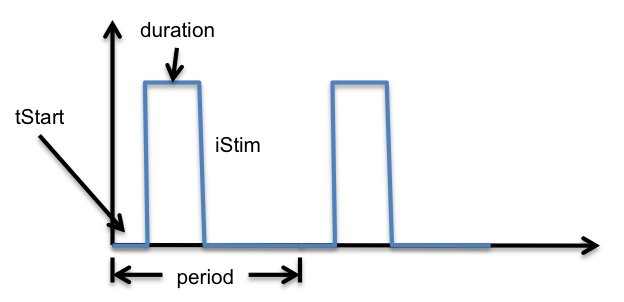
\includegraphics{graphics/pulseTrain.png}}
  \caption{Periodic pulse train.}
  \label{fig:grid_comparsion}
\end{figure}

\subsection{Producing data for read results with cardioid}
The proceedure for producing the appropriate data is as follows. Given a cardioid regular
finite element grid, an auxiliary mesh may be formed were a small sample (1:1000)
points are seleted from the grid. As this mesh is for visualisation only, it is not
constrained to the cubic geometry. However each nodal point on the polyhedral mesh
will correspond to a evaluation point within the finite element grid. In order
to use this auxiliary grid with cardioid we must extract information, from the cardioid
finite element grid, at the relevant points to the auxiliary grid, followed by
associating this data with the auxiliary grid in a vtk data file.

To conduct this procedure first we must construct a 
\verb|sensor.txt| file. This file is a whitespace separated lists of the mapping from the 'vtk datafile
indices to the PIO GIDs. I.e. a list of PIO GIDs in order of increasing vtk point
index.

The sensor file is used generate output from cardioid. Two groups of methods are employed to output. The first
based on the \verb|snapshotCellList|:
\begin{verbatim}
simulate SIMULATE
{
   snapshotRate = 400;
   snapshotCellList = sensor.txt;
}
\end{verbatim}
The \verb|object.data| snippet above will output membrane voltage, region (MPI rank)
and cell type for each of the selected nodes every 400 timesteps. The data is stored
in \verb|./snapshot.`timestep'/anatomy#*|. A second example for calculating membrane
voltage spatial gradient follows where the data is stored within  \verb|./snapshot.`timestep'/coarsened_anatomy#*|.
\begin{verbatim}
simulate SIMULATE
{
   sensor = myGradient;
}

myGradient SENSOR
{
   method = gradientVoronoiCoarsening;
   cellList = "sensor.txt";
   maxDistance = 0.19 mm;
   printRate = 400;
   evalRate = 400;
}
\end{verbatim}

\subsection{Employing |read\_results|}
Given data produced as described in the previous section \verb|read\_results| may
be used in the case directory. In addition to the snapshot directory two files are
needed in the case directory with fixed names: \verb|sensor.txt| as described above
and \verb|wedge.vtk|, the corresponding VTK UnstructuredGrid.

Two approaches may be taken calling read\_results:
\begin{verbatim}
./read\_results -n anatomy# 

./read\_results -j a_json_file.json
\end{verbatim}
The first approach (using the \verb|-n| flag), processes all of the snapshot
directories in sequential order, reading the files within each snapshot directory
prefixed with \verb|anatomy#|.

The second approach uses a json file to selectively index the snapshot directories
to process. The json block following describes which snapshot directories it will
process based on timestep index.
\begin{verbatim}
{
    "read_results": {
    	"start_index" : 400,
    	"stride_length": 400,
    	"end_index": 1200,
	"prefix": "anatomy#"
    }
}
\end{verbatim}




\end{document}
